\documentclass[a4paper]{article}

\usepackage[portuguese]{babel}
\usepackage[utf8]{inputenc}
\usepackage[T1]{fontenc}

\newcommand{\documentTitle}{Ray-Tracer with Photon Mapping} %Macro definition
\newcommand{\documentAuthors}{João Rafael (2008111876, jprafael@student.dei.uc.pt) \and José Ribeiro (2008112181, jbaia@student.dei.uc.pt)} %Macro definition

\title{\documentTitle}
\author{\documentAuthors{}}

\usepackage{hyperref}
\hypersetup{
	pdftitle = \documentTitle
	,pdfauthor = \documentAuthors
	,pdfsubject = {Computer Graphics Project Final Report}
	,pdfkeywords = {Computer Graphics Project} {Photon Mapping} {Raytracing}
	,pdfborder = {0 0 0}
}

\usepackage{subfig}
\usepackage{amsmath}
\usepackage{wrapfig}
\usepackage{array}
\usepackage{anysize}
\usepackage{lscape}
\usepackage[pdftex]{graphicx}
\usepackage{longtable}
\usepackage{multirow}
\usepackage[table]{xcolor}
\usepackage{caption}

\marginsize{3.5cm}{3.5cm}{3cm}{3cm}

\makeatletter

\begin{document}

\renewcommand{\figurename}{Figure}
\renewcommand{\contentsname}{Contents}

\maketitle
\cleardoublepage

\tableofcontents
\cleardoublepage

\setlength{\parindent}{1cm}
\setlength{\parskip}{0.3cm}

\section{Introduction}
\indent \indent O \emph{ray-tracing} é uma técnica de renderização de imagens que tem como principal objectivo o fotorealismo.
O funcionamento básico deste consiste na projecção de raios através de uma grelha no espaço que representa o ecrã.
Estes raios são reflectidos e refractados até atingirem uma superfície difusa. Quando tal acontece a cor do raio é
calculada através da proximidade às luzes e da cor do objecto.

\indent O \emph{photon-mapping} é uma melhoria deste método. Numa fase de pré-processamento são emitidos fotões
das luzes presentes na cena. Esses fotões são estocasticamente distribuídos, reflectidos, refractados e absorvidos,
sendo apenas armazenados quando são reflectidos de forma difusa, pois apenas estes importam na fase seguinte.
Posteriormente, na fase de \emph{ray-tracing}, a cor dos raios é obtida através da soma da cor dos fotões mais próximos.
O pré-processamento só é efectuado uma vez por cena, podendo o \emph{photon-map} ser reutilizado para a renderização através de outras câmeras.

\indent Este método permite obter maior realismo, em particular em relação à iluminação resultante, nomeadamente cáusticas e inter-reflecção difusa.

\cleardoublepage
\section{Implementation}
\subsection{Performance}
\indent \indent Desde o início do projecto que um aspecto fulcral nas decisões tomadas foi a performance. Com este objectivo em mente,
e de forma a tentar manter o código estruturado e modular, a linguagem de programação escolhida foi o \texttt{C++}. 

\indent Também com o mesmo propósito, decidimos integrar duas bibliotecas \emph{open-source}:

\begin{description}
	\item[libkdtree++ (http://libkdtree.alioth.debian.org/)] \hfill \\
		Implementação de uma kD-Tree balanceada, mantida por Paul Harris.
		Foi utilizada com o intuito	de armazenar os fotões e permitir pesquisas (\emph{range queries}) rápidas.
	\item[OpenMP (http://openmp.org/)] \hfill \\
		Após a projecção dos fotões e dos raios primários, a restante propagação dos raios é uma tarefa altamente paralelizável.
		Assim, de forma a tirar proveito dos recursos existentes nos processadores actuais, decidimos utilizar OpenMP, uma biblioteca
		de programação concorrente para \texttt{C/C++ e Fortran}.
\end{description}

\subsection{Scene loading}
\indent \indent Para permitir a criação de cenas a renderizar sem a necessidade de recompilação do código decidimos implementar um formato de descrição
de cena que fosse facilmente \emph{parsable} e de simples manutenção. Após indecisão entre os formatos de descrição de objectos de \texttt{Lua} e \texttt{JSON},
optámos por \texttt{JSON}, dado que as \texttt{APIs} disponíveis para esta linguagem não necessitam de recorrer a bibliotecas externas.

\indent Descreve-se de seguida o formato da cena:
\begin{description}
	\item[Scene] \hfill
		\begin{description}
			\item[Materials] \hfill \\
				\texttt{Array} de \texttt{Objects} correspondentes à classe \texttt{Material}, compostos pelos seguintes parâmetros:
				\begin{description}
					\item[color] \hfill \\
						Cor do material.
					\item[roughness] \hfill \\
						Valor de 0 a 1, correspondente ao inverso do grau de polimento.
					\item[absorvance] \hfill \\
						Valor de 0 a 1, correspondente à absorvância do material; isto é, a fracção de luz que atinge o material e é absorvida por este.
					\item[emittance] \hfill \\
						Valor de 0 a $\infty$, correspondente à luminosidade da \texttt{Primitive}.
					\item[n] \hfill \\
						Valor de 0 a $\infty$, correspondente ao índice de refracção do material; isto é, o valor relativo da velocidade da luz no meio em relação
						à velocidade da luz no vácuo.
				\end{description}

				É necessário pelo menos um \texttt{Material}.
			\item[Lights] \hfill \\
				\texttt{Array} de \texttt{Objects} correspondentes à classe \texttt{Primitive}.
				Os seus parâmetros dependem do tipo de \texttt{Primitive} (ver secção \ref{sec:primitives}).
				Apenas os objectos presentes nesta secção serão usados no cálculo do mapa de fotões. \\
				É necessário pelo menos uma \texttt{Primitive} do tipo \texttt{Light}.
			\item[Primitives (obrigatório)] \hfill \\
				\texttt{Array} de \texttt{Objects} correspondentes à classe \texttt{Primitive}.
				Os seus parâmetros dependem do tipo de \texttt{Primitive} (ver secção \ref{sec:primitives}).
		\end{description}
	\item[Cameras] \hfill \\
		\texttt{Array} de \texttt{Objects} correspondentes à classe \texttt{Camera}.
		Os seus parâmetros são descritos de seguida:
		\begin{description}
			\item[origin] \hfill \\
				Ponto correspondente ao ponto de origem da câmera.
			\item[direction] \hfill \\
				Vector normalizado correspondente à direcção da câmera.
			\item[top] \hfill \\
				Vector normalizado correspondente ao \emph{top} da câmera (orientação).
			\item[fovy] \hfill \\
				Valor em graus correspondente ao \textit{field-of-view} da câmera.
			\item[width] \hfill \\
				Valor em píxeis, correspondente à largura da imagem final.
			\item[height] \hfill \\
				Valor em píxeis, correspondente à altura da imagem final.
			\item[filename] \hfill \\
				Nome do ficheiro de \textit{output} da imagem \texttt{.ppm}.
		\end{description}

	\item[Engine (opcional)] \hfill
		\begin{description}
			\item[Configurations (opcional)] \hfill \\
				Objecto correspondente aos parâmetros referentes ao \emph{Engine}.
				\begin{description}
					\item[MAX\_PHOTONS (opcional)] \hfill \\
						Valor de 1 a $\infty$, correspondente ao número máximo de fotões em cena.
					\item[MAX\_PHOTON\_BOUNCE (opcional)] \hfill \\
						Valor de 1 a $\infty$, correspondente ao limite de recursividade relativo à reflexão de fotões.
					\item[MAX\_RAY\_BOUNCE (opcional)] \hfill \\
						Valor de 1 a $\infty$, correspondente ao limite de recursividade relativo à reflexão de raios.
					\item[MAX\_GATHER\_DISTANCE (opcional)] \hfill \\
						Valor de 0 a $\infty$, correspondente ao raio de influência de um fotão.
					\item[EXPOSURE (opcional)] \hfill \\
						Valor de 0 a $\infty$, correspondente à luminosidade associada a cada fotão.
					\item[EPS (opcional)] \hfill \\
						Valor de 0 a $\infty$, correspondente à diferença mínima para dois números de vírgula flutoante serem considerados diferentes.
					\item[ANTIALIAS\_THRESHOLD (opcional)] \hfill \\
						Valor de 0 a 1, correspondente ao nível de energia a partir do qual é feita oversamplagem de um dado píxel.
				\end{description}
		\end{description}
\end{description}

O nó \texttt{Engine} foi criado como uma lista de \texttt{Objects} para permitir a possível extensibilidade do formato de descrição.

\cleardoublepage
\subsection{Primitives}
\label{sec:primitives}
\indent \indent Um processo importante na construção de um \emph{ray-tracer}, é a implementação de primitivas que componham a cena.
Para cada tipo de primitiva, é necessário implementar as seguintes propriedade e métodos:

\begin{description}
	\item [\texttt{area()}] \hfill \\
		Área total da superfície da primitiva.

	\item [\texttt{intersect(ray)}] \hfill \\
		Método que calcula, se existir, o ponto de intersecção entre o raio e a primitiva, que esteja localizado
		mais próximo da origem do raio.

	\item [\texttt{normal(point)}] \hfill \\
		Método que devolve a normal à superfície da primitiva num ponto.

	\item [\texttt{randomPhoton()}] \hfill \\
		Método que cria um fotão á superfície da primitiva, com uma direcção pseudo-aleatória.
 
\end{description}

\subsubsection{Sphere}
\indent \indent Uma esfera definida através do ponto central e do raio.   

\subsubsection{Plane}
\indent \indent Um plano definido através de um ponto pertencente e de um vector normal a este.
Uma vez que a sua superfície é por definição infinita, esta não pode servir de fonte de luz.

\subsubsection{Quad}
\indent \indent Um quadrilátero definido por 3 dos 4 vértices, sendo o último calculado como indica a figura.
\begin{center}
	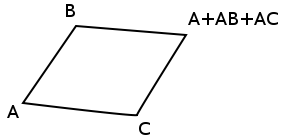
\includegraphics[scale=0.50]{images/quad.png}
	\captionof{figure}{Quadrilateral}
	\label{fig:quad}
\end{center}

\subsubsection{Box}
\indent \indent Uma caixa definida por um dos vértices desta, e 3 vectores correspondentes a cada uma das 
arestas que contém este vértice.

\cleardoublepage
\subsection{Reflection}

\begin{center}
	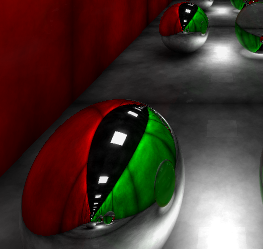
\includegraphics[scale=0.50]{images/reflection.png}
	\captionof{figure}{Reflection}
	\label{fig:reflection}
\end{center}

\indent No modelo físico a componente difusa de um material corresponde à reflecção da luz numa superfície
que contém micro-ruído. A luz ao insidir nesta superfície é espalhada para várias direcções. 

\indent Este fenómeno é facilmente reproduzido na fase de \emph{photon-mapping}.
No entanto, na fase de \emph{ray-tracing} seria necessário projectar, para cada reflecção, vários raios, o que
é computacionalmente muito exigente, pelo que para este caso é utilizada outro método.

\subsubsection{Specular}
\indent \indent Tal como indicado, caso a reflecção seja especular os raios (e fotões) obtém uma nova direcção,
calculada através da normal à superfície, e a cor provém destes. 

\subsubsection{Diffuse}
\indent Caso a reflecção seja difusa a cor é inferida a partir da radiosidade local,
isto é, pela intensidade\footnote{A importância de cada fotão depende do coseno do ângulo formado entre a sua direcção e a da normal à superfície} dos fotões perto do ponto de reflecção.

\begin{displaymath}
	Radiosity = \frac{E}{\pi r^{2}} \sum \limits_{p \in P}{\max(0, \vec{N} \cdot \vec{d_{p}})}
\end{displaymath}

\indent Onde $E$ é a intensidade de luz de um fotão (\emph{exposure}), $r$ é o raio de influência de um fotão,
$P$ é o conjunto de fotões a uma distância máxima $r$ do ponto, $\vec{N}$ é o vector normal à superfície
e $\vec{d_{p}}$ é a direcção do fotão $p$. 

\indent Um efeito visível com esta técnica é o \emph{color bleeding}: transferência de cor entre duas superfícies
através de reflecções difusas.

\cleardoublepage
\subsection{Refraction}
\begin{center}
	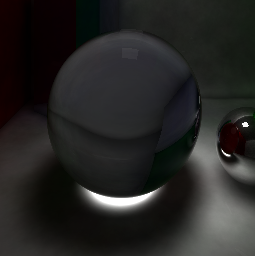
\includegraphics[scale=0.50]{images/caustics.png}
	\captionof{figure}{Caustics}
	\label{fig:caustics}
\end{center}

\indent A refracção é um efeito visível quando a luz muda entre meios com diferentes densidades.
Este efeito caracteriza-se pela diferença entre a direcção do raio incidente e a direcção do raio emergente. 
Desta forma a sua implementação adequa-se na sua totalidade ao paradigma de ray-tracing.

\subsubsection{Attenuation}
\indent \indent Ao atravessar um material translúcido, parte da energia de um fotão é absorvida. De forma análoga,
um raio ao passar pelo mesmo material obtém parte da sua cor através da cor do material.

\subsubsection{Caustics}
\indent \indent Ao sofrer sucessivas refracções, os fotões tendem a convergir, dando origem a cáusticas luminosas.
Este efeito depende apenas do \emph{photon-mapping} pelo que sem ele (i.e.: com \emph{ray-tracing} puro)
não são observáveis.

\cleardoublepage
\subsection{Anti-Alliasing}
\begin{center}
	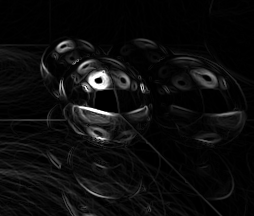
\includegraphics[scale=0.50]{images/sobel.png}
	\captionof{figure}{Sobel's operator result}
	\label{fig:sobel}
\end{center}

\indent Um método de obter melhores resultados é através da sobresamplagem da imagem (ex.: projectando
4 raios por píxel ao invés de apenas 1). No entanto este método é computacionalmente dispendioso pelo que não
deve ser aplicado à imagem na sua totalidade.

\indent Desta forma, para selecionar quais os píxeis que têm mais importância, é utilizado o operador de Sobel
para calcular a energia associada a cada pixel. Após este cálculo, apenas aqueles com energia superior a um limiar
são sobresamplados.

\cleardoublepage
\section{Gallery}
\subsection{Evolution}
\begin{center}
	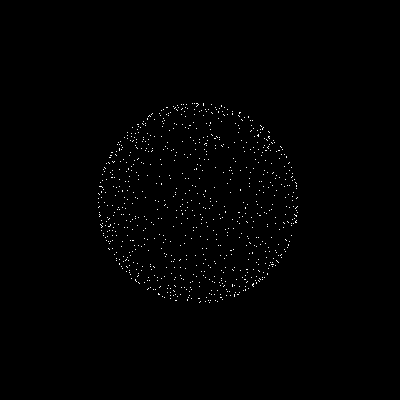
\includegraphics[scale=0.50]{images/gallery/photon_projection.png}
	\captionof{figure}{Initial projection of photons on the surface of a sphere shapped light.}
	\label{fig:photon_projection}
\end{center}

\begin{center}
	
\includegraphics[scale=0.50]{images/gallery/ray_casting.png}
	\captionof{figure}{First projection and intersection of rays and spheres.}
	\label{fig:ray_projection}
\end{center}

\begin{center}
	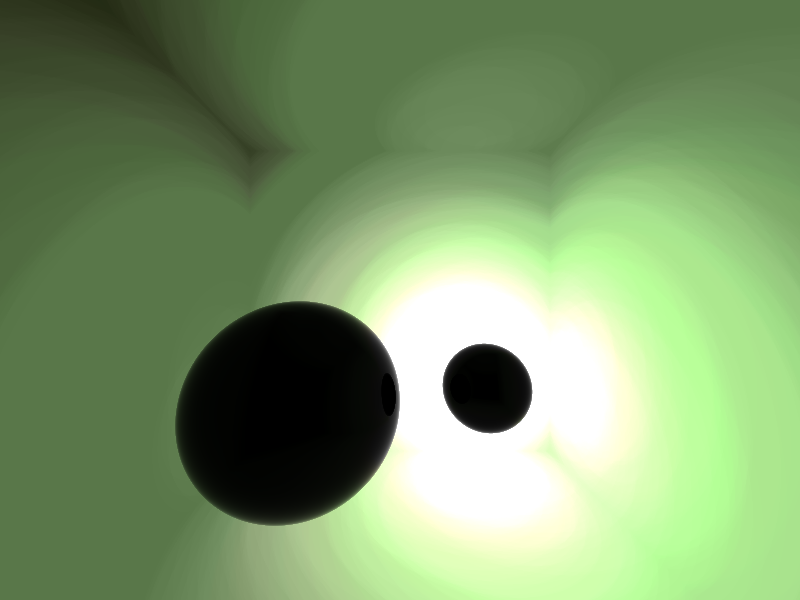
\includegraphics[scale=0.45]{images/gallery/diffuse.png}
	\captionof{figure}{Radiosity gathering of photons emitted by a white light (here still rendered black).}
	\label{fig:diffuse}
\end{center}

\begin{center}
	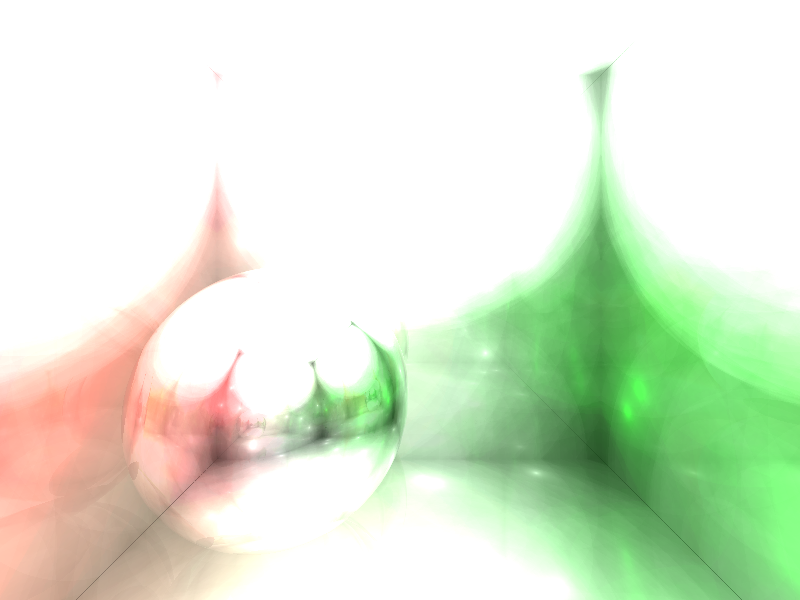
\includegraphics[scale=0.45]{images/gallery/reflection.png}
	\captionof{figure}{Over-exposed image of a scene showing reflections.}
	\label{fig:reflections}
\end{center}

\begin{center}
	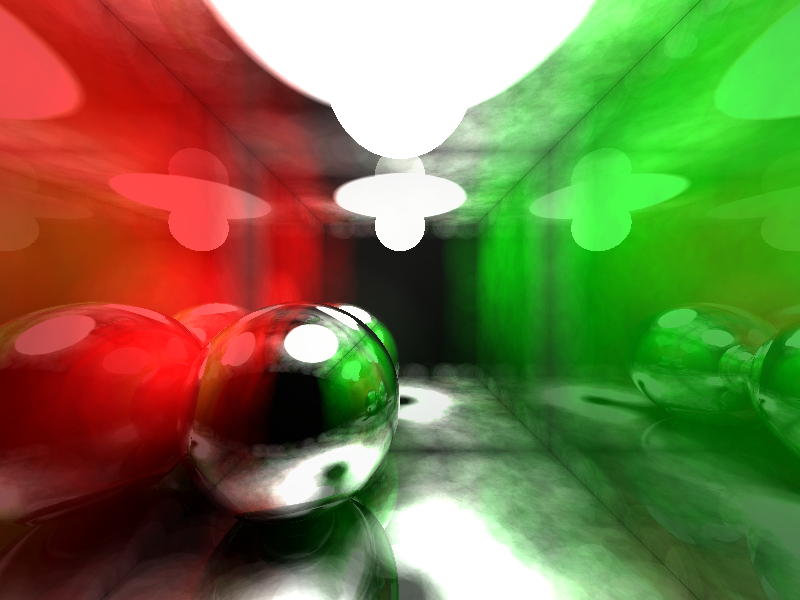
\includegraphics[scale=0.45]{images/gallery/color_bleed.png}
	\captionof{figure}{Exagerated color bleeding effect.}
	\label{fig:caustics}
\end{center}

\begin{center}
	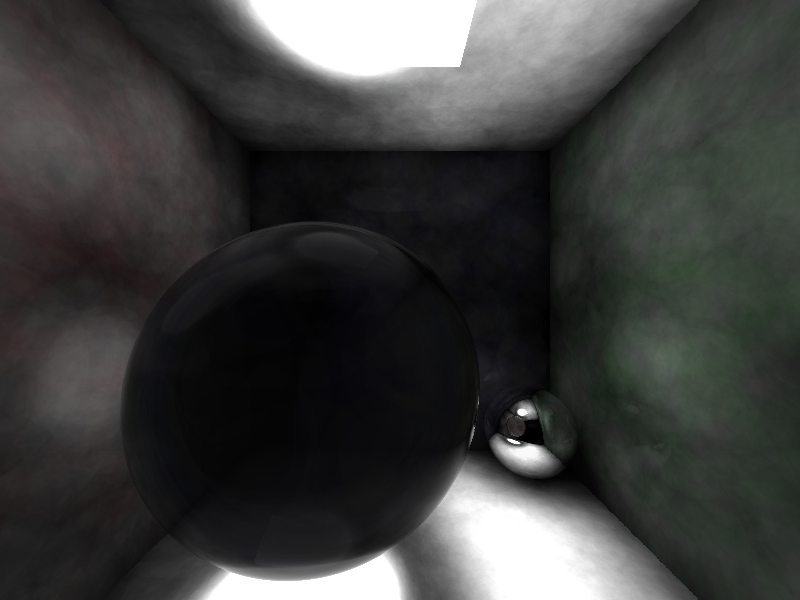
\includegraphics[scale=0.45]{images/gallery/caustics.png}
	\captionof{figure}{Light refraction producing strong caustics.}
	\label{fig:caustics}
\end{center}

\begin{center}
	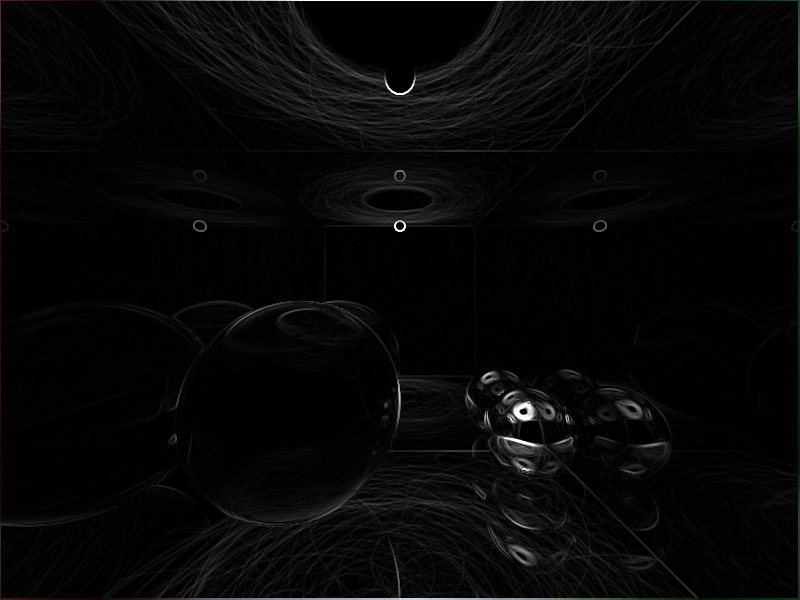
\includegraphics[scale=0.45]{images/gallery/sobel.png}
	\captionof{figure}{Application of Sobel's edge detection operator.}
	\label{fig:sobel}
\end{center}

\cleardoublepage
\subsection{Final}

\begin{center}
	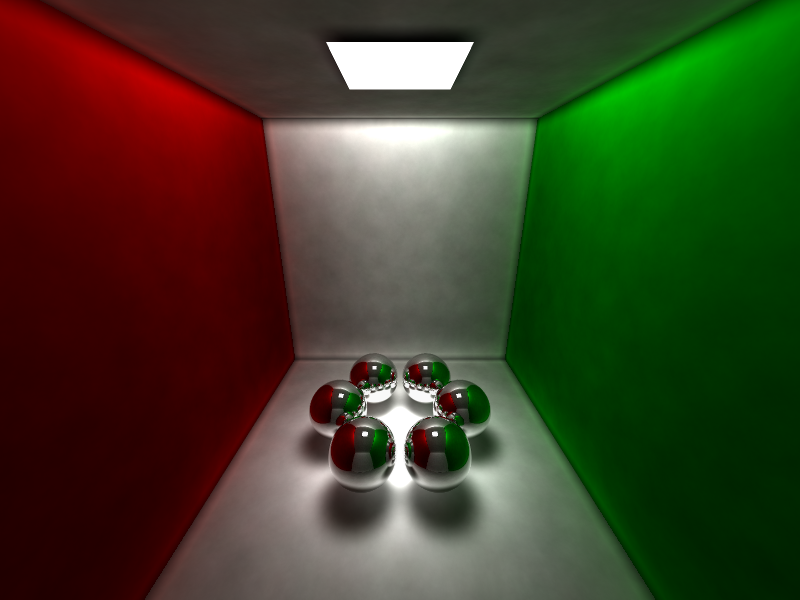
\includegraphics[scale=0.43]{images/gallery/balls.png}
	\captionof{figure}{An adaptation of the Cornell box with 6 metallic spheres.}
	\label{fig:balls}
\end{center}

\begin{center}
	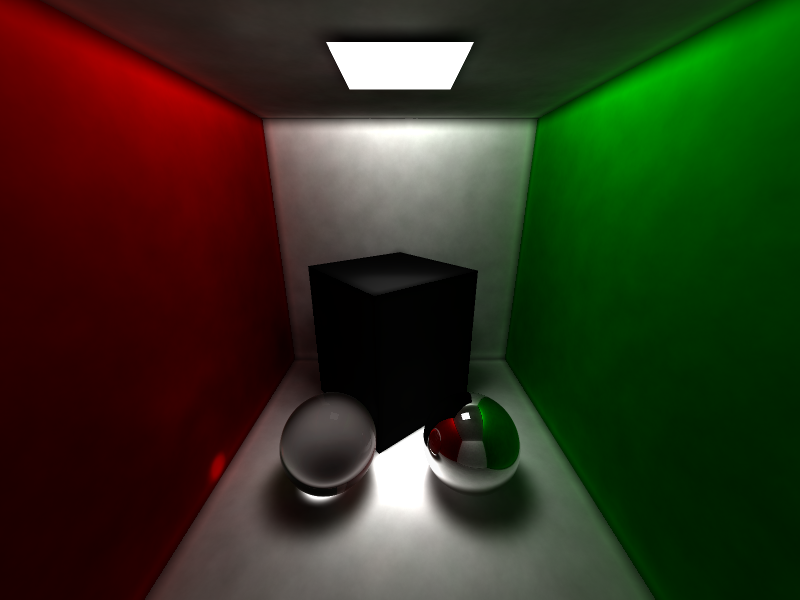
\includegraphics[scale=0.43]{images/gallery/mixed.png}
	\captionof{figure}{Scene showing mixed proprieties and primitives.}
	\label{fig:mixed}
\end{center}

\begin{center}
	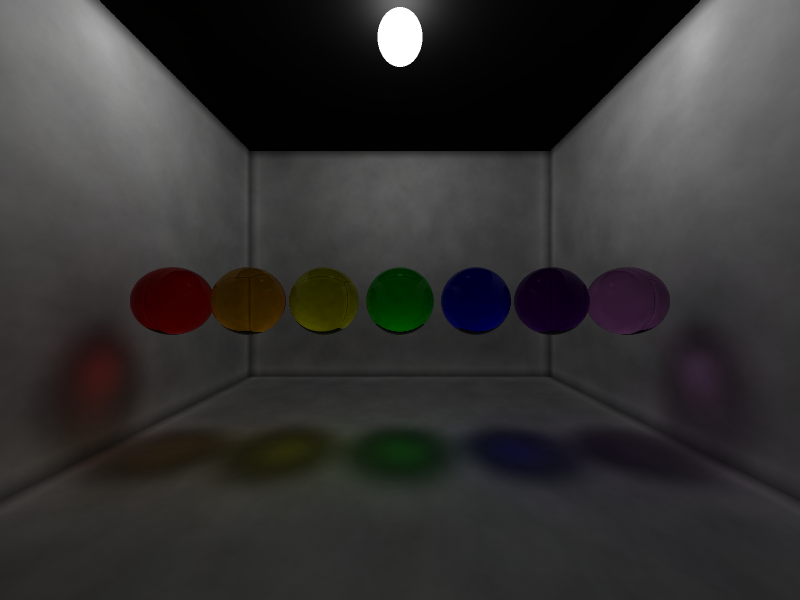
\includegraphics[scale=0.43]{images/gallery/rainbow.png}
	\captionof{figure}{A scene with 7 colored glass spheres, with the colors of the rainbow.}
	\label{fig:mixed}
\end{center}

% TODO Mirror box
\end{document}
